% Created by tikzDevice version 0.12.3.1 on 2021-09-17 14:35:11
% !TEX encoding = UTF-8 Unicode
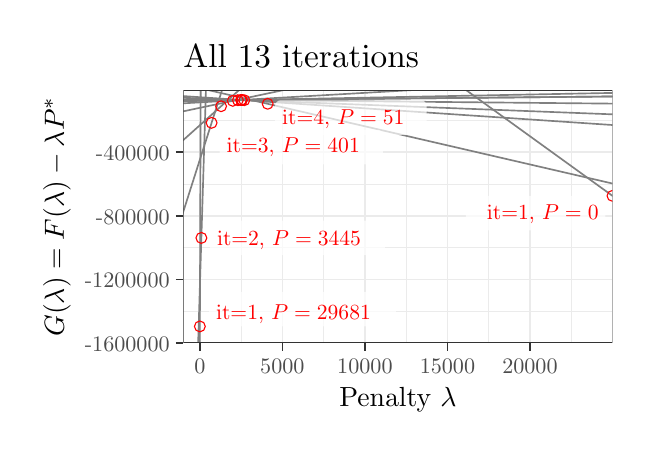
\begin{tikzpicture}[x=1pt,y=1pt]
\definecolor{fillColor}{RGB}{255,255,255}
\path[use as bounding box,fill=fillColor,fill opacity=0.00] (0,0) rectangle (216.81,144.54);
\begin{scope}
\path[clip] (  0.00,  0.00) rectangle (216.81,144.54);
\definecolor{drawColor}{RGB}{255,255,255}
\definecolor{fillColor}{RGB}{255,255,255}

\path[draw=drawColor,line width= 0.6pt,line join=round,line cap=round,fill=fillColor] (  0.00,  0.00) rectangle (216.81,144.54);
\end{scope}
\begin{scope}
\path[clip] ( 56.26, 30.61) rectangle (211.31,121.94);
\definecolor{fillColor}{RGB}{255,255,255}

\path[fill=fillColor] ( 56.26, 30.61) rectangle (211.31,121.94);
\definecolor{drawColor}{gray}{0.92}

\path[draw=drawColor,line width= 0.3pt,line join=round] ( 56.26, 42.09) --
	(211.31, 42.09);

\path[draw=drawColor,line width= 0.3pt,line join=round] ( 56.26, 65.07) --
	(211.31, 65.07);

\path[draw=drawColor,line width= 0.3pt,line join=round] ( 56.26, 88.05) --
	(211.31, 88.05);

\path[draw=drawColor,line width= 0.3pt,line join=round] ( 56.26,111.02) --
	(211.31,111.02);

\path[draw=drawColor,line width= 0.3pt,line join=round] ( 77.13, 30.61) --
	( 77.13,121.94);

\path[draw=drawColor,line width= 0.3pt,line join=round] (106.95, 30.61) --
	(106.95,121.94);

\path[draw=drawColor,line width= 0.3pt,line join=round] (136.77, 30.61) --
	(136.77,121.94);

\path[draw=drawColor,line width= 0.3pt,line join=round] (166.58, 30.61) --
	(166.58,121.94);

\path[draw=drawColor,line width= 0.3pt,line join=round] (196.40, 30.61) --
	(196.40,121.94);

\path[draw=drawColor,line width= 0.3pt,line join=round] (211.31, 30.61) --
	(211.31,121.94);

\path[draw=drawColor,line width= 0.6pt,line join=round] ( 56.26, 30.61) --
	(211.31, 30.61);

\path[draw=drawColor,line width= 0.6pt,line join=round] ( 56.26, 53.58) --
	(211.31, 53.58);

\path[draw=drawColor,line width= 0.6pt,line join=round] ( 56.26, 76.56) --
	(211.31, 76.56);

\path[draw=drawColor,line width= 0.6pt,line join=round] ( 56.26, 99.53) --
	(211.31, 99.53);

\path[draw=drawColor,line width= 0.6pt,line join=round] ( 62.22, 30.61) --
	( 62.22,121.94);

\path[draw=drawColor,line width= 0.6pt,line join=round] ( 92.04, 30.61) --
	( 92.04,121.94);

\path[draw=drawColor,line width= 0.6pt,line join=round] (121.86, 30.61) --
	(121.86,121.94);

\path[draw=drawColor,line width= 0.6pt,line join=round] (151.68, 30.61) --
	(151.68,121.94);

\path[draw=drawColor,line width= 0.6pt,line join=round] (181.49, 30.61) --
	(181.49,121.94);
\definecolor{drawColor}{gray}{0.50}

\path[draw=drawColor,line width= 0.6pt,line join=round] ( 59.05,-867.24) -- ( 65.64,1011.78);

\path[draw=drawColor,line width= 0.6pt,line join=round] (-98.79,307.79) -- (366.36,-28.23);

\path[draw=drawColor,line width= 0.6pt,line join=round] ( 33.94,-867.24) -- ( 91.82,1011.78);

\path[draw=drawColor,line width= 0.6pt,line join=round] (-98.79,-408.73) -- (353.60,1011.78);

\path[draw=drawColor,line width= 0.6pt,line join=round] (-98.79,159.91) -- (366.36, 52.38);

\path[draw=drawColor,line width= 0.6pt,line join=round] (-98.79,-34.94) -- (366.36,381.73);

\path[draw=drawColor,line width= 0.6pt,line join=round] (-98.79, 81.46) -- (366.36,180.02);

\path[draw=drawColor,line width= 0.6pt,line join=round] (-98.79,130.27) -- (366.36, 98.91);

\path[draw=drawColor,line width= 0.6pt,line join=round] (-98.79,108.24) -- (366.36,135.12);

\path[draw=drawColor,line width= 0.6pt,line join=round] (-98.79,114.99) -- (366.36,123.95);

\path[draw=drawColor,line width= 0.6pt,line join=round] (-98.79,125.17) -- (366.36,107.25);

\path[draw=drawColor,line width= 0.6pt,line join=round] (-98.79,120.08) -- (366.36,115.60);

\path[draw=drawColor,line width= 0.6pt,line join=round] (-98.79,116.69) -- (366.36,121.17);

\path[draw=drawColor,line width= 0.6pt,line join=round] (-98.79,116.69) -- (366.36,121.17);
\definecolor{fillColor}{RGB}{255,255,255}

\path[fill=fillColor,fill opacity=0.70] ( 67.58, 36.59) --
	(131.04, 36.59) --
	(130.96, 36.59) --
	(131.27, 36.60) --
	(131.59, 36.67) --
	(131.89, 36.78) --
	(132.16, 36.94) --
	(132.41, 37.14) --
	(132.62, 37.38) --
	(132.80, 37.65) --
	(132.92, 37.95) --
	(133.00, 38.26) --
	(133.02, 38.58) --
	(133.02, 38.58) --
	(133.02, 47.08) --
	(133.02, 47.08) --
	(133.00, 47.40) --
	(132.92, 47.71) --
	(132.80, 48.00) --
	(132.62, 48.27) --
	(132.41, 48.51) --
	(132.16, 48.71) --
	(131.89, 48.87) --
	(131.59, 48.99) --
	(131.27, 49.05) --
	(131.04, 49.06) --
	( 67.58, 49.06) --
	( 67.82, 49.05) --
	( 67.50, 49.06) --
	( 67.19, 49.02) --
	( 66.88, 48.94) --
	( 66.59, 48.80) --
	( 66.33, 48.62) --
	( 66.10, 48.40) --
	( 65.90, 48.14) --
	( 65.75, 47.86) --
	( 65.65, 47.55) --
	( 65.60, 47.24) --
	( 65.60, 47.08) --
	( 65.60, 38.58) --
	( 65.60, 38.74) --
	( 65.60, 38.42) --
	( 65.65, 38.10) --
	( 65.75, 37.80) --
	( 65.90, 37.51) --
	( 66.10, 37.26) --
	( 66.33, 37.04) --
	( 66.59, 36.85) --
	( 66.88, 36.72) --
	( 67.19, 36.63) --
	( 67.50, 36.59) --
	cycle;
\end{scope}
\begin{scope}
\path[clip] ( 56.26, 30.61) rectangle (211.31,121.94);
\definecolor{drawColor}{RGB}{255,0,0}

\node[text=drawColor,anchor=base west,inner sep=0pt, outer sep=0pt, scale=  0.78] at ( 68.09, 39.16) {it=1, $P=29681$};
\definecolor{fillColor}{RGB}{255,255,255}

\path[fill=fillColor,fill opacity=0.70] (160.34, 71.30) --
	(206.80, 71.30) --
	(206.72, 71.30) --
	(207.04, 71.31) --
	(207.35, 71.38) --
	(207.65, 71.49) --
	(207.93, 71.65) --
	(208.18, 71.85) --
	(208.39, 72.09) --
	(208.56, 72.36) --
	(208.69, 72.66) --
	(208.76, 72.97) --
	(208.79, 73.29) --
	(208.79, 73.29) --
	(208.79, 81.79) --
	(208.79, 81.79) --
	(208.76, 82.11) --
	(208.69, 82.42) --
	(208.56, 82.71) --
	(208.39, 82.98) --
	(208.18, 83.22) --
	(207.93, 83.42) --
	(207.65, 83.58) --
	(207.35, 83.70) --
	(207.04, 83.76) --
	(206.80, 83.77) --
	(160.34, 83.77) --
	(160.58, 83.76) --
	(160.26, 83.77) --
	(159.95, 83.73) --
	(159.64, 83.65) --
	(159.35, 83.51) --
	(159.09, 83.33) --
	(158.86, 83.11) --
	(158.66, 82.85) --
	(158.51, 82.57) --
	(158.41, 82.26) --
	(158.36, 81.95) --
	(158.36, 81.79) --
	(158.36, 73.29) --
	(158.36, 73.44) --
	(158.36, 73.13) --
	(158.41, 72.81) --
	(158.51, 72.51) --
	(158.66, 72.22) --
	(158.86, 71.97) --
	(159.09, 71.75) --
	(159.35, 71.56) --
	(159.64, 71.43) --
	(159.95, 71.34) --
	(160.26, 71.30) --
	cycle;
\end{scope}
\begin{scope}
\path[clip] ( 56.26, 30.61) rectangle (211.31,121.94);
\definecolor{drawColor}{RGB}{255,0,0}

\node[text=drawColor,anchor=base east,inner sep=0pt, outer sep=0pt, scale=  0.78] at (206.29, 75.35) {it=1, $P=0$};
\definecolor{fillColor}{RGB}{255,255,255}

\path[fill=fillColor,fill opacity=0.70] ( 67.91, 62.33) --
	(127.12, 62.33) --
	(127.04, 62.34) --
	(127.36, 62.35) --
	(127.67, 62.41) --
	(127.97, 62.53) --
	(128.25, 62.69) --
	(128.49, 62.89) --
	(128.70, 63.13) --
	(128.88, 63.40) --
	(129.00, 63.69) --
	(129.08, 64.00) --
	(129.10, 64.32) --
	(129.10, 64.32) --
	(129.10, 72.82) --
	(129.10, 72.82) --
	(129.08, 73.14) --
	(129.00, 73.45) --
	(128.88, 73.75) --
	(128.70, 74.02) --
	(128.49, 74.26) --
	(128.25, 74.46) --
	(127.97, 74.62) --
	(127.67, 74.73) --
	(127.36, 74.80) --
	(127.12, 74.81) --
	( 67.91, 74.81) --
	( 68.15, 74.80) --
	( 67.83, 74.81) --
	( 67.51, 74.77) --
	( 67.21, 74.68) --
	( 66.92, 74.55) --
	( 66.66, 74.36) --
	( 66.42, 74.14) --
	( 66.23, 73.89) --
	( 66.08, 73.60) --
	( 65.98, 73.30) --
	( 65.93, 72.98) --
	( 65.92, 72.82) --
	( 65.92, 64.32) --
	( 65.93, 64.48) --
	( 65.93, 64.16) --
	( 65.98, 63.85) --
	( 66.08, 63.54) --
	( 66.23, 63.26) --
	( 66.42, 63.00) --
	( 66.66, 62.78) --
	( 66.92, 62.60) --
	( 67.21, 62.46) --
	( 67.51, 62.37) --
	( 67.83, 62.34) --
	cycle;
\end{scope}
\begin{scope}
\path[clip] ( 56.26, 30.61) rectangle (211.31,121.94);
\definecolor{drawColor}{RGB}{255,0,0}

\node[text=drawColor,anchor=base west,inner sep=0pt, outer sep=0pt, scale=  0.78] at ( 68.42, 65.65) {it=2, $P=3445$};
\definecolor{fillColor}{RGB}{255,255,255}

\path[fill=fillColor,fill opacity=0.70] ( 71.39, 95.18) --
	(126.35, 95.18) --
	(126.27, 95.18) --
	(126.59, 95.19) --
	(126.90, 95.26) --
	(127.20, 95.37) --
	(127.48, 95.53) --
	(127.72, 95.73) --
	(127.94, 95.97) --
	(128.11, 96.24) --
	(128.23, 96.54) --
	(128.31, 96.85) --
	(128.33, 97.17) --
	(128.33, 97.17) --
	(128.33,105.67) --
	(128.33,105.67) --
	(128.31,105.99) --
	(128.23,106.30) --
	(128.11,106.59) --
	(127.94,106.86) --
	(127.72,107.10) --
	(127.48,107.30) --
	(127.20,107.46) --
	(126.90,107.58) --
	(126.59,107.64) --
	(126.35,107.65) --
	( 71.39,107.65) --
	( 71.63,107.64) --
	( 71.31,107.65) --
	( 70.99,107.61) --
	( 70.69,107.53) --
	( 70.40,107.39) --
	( 70.13,107.21) --
	( 69.90,106.99) --
	( 69.71,106.73) --
	( 69.56,106.45) --
	( 69.46,106.14) --
	( 69.41,105.83) --
	( 69.40,105.67) --
	( 69.40, 97.17) --
	( 69.41, 97.33) --
	( 69.41, 97.01) --
	( 69.46, 96.69) --
	( 69.56, 96.39) --
	( 69.71, 96.10) --
	( 69.90, 95.85) --
	( 70.13, 95.63) --
	( 70.40, 95.44) --
	( 70.69, 95.31) --
	( 70.99, 95.22) --
	( 71.31, 95.18) --
	cycle;
\end{scope}
\begin{scope}
\path[clip] ( 56.26, 30.61) rectangle (211.31,121.94);
\definecolor{drawColor}{RGB}{255,0,0}

\node[text=drawColor,anchor=base west,inner sep=0pt, outer sep=0pt, scale=  0.78] at ( 71.90, 99.53) {it=3, $P=401$};
\definecolor{fillColor}{RGB}{255,255,255}

\path[fill=fillColor,fill opacity=0.70] ( 91.44,105.80) --
	(142.15,105.80) --
	(142.07,105.80) --
	(142.39,105.81) --
	(142.70,105.87) --
	(143.00,105.99) --
	(143.28,106.15) --
	(143.53,106.35) --
	(143.74,106.59) --
	(143.91,106.86) --
	(144.03,107.15) --
	(144.11,107.47) --
	(144.14,107.78) --
	(144.14,107.78) --
	(144.14,116.29) --
	(144.14,116.29) --
	(144.11,116.60) --
	(144.03,116.92) --
	(143.91,117.21) --
	(143.74,117.48) --
	(143.53,117.72) --
	(143.28,117.92) --
	(143.00,118.08) --
	(142.70,118.19) --
	(142.39,118.26) --
	(142.15,118.27) --
	( 91.44,118.27) --
	( 91.68,118.26) --
	( 91.36,118.27) --
	( 91.05,118.23) --
	( 90.74,118.14) --
	( 90.45,118.01) --
	( 90.19,117.83) --
	( 89.96,117.60) --
	( 89.76,117.35) --
	( 89.61,117.06) --
	( 89.51,116.76) --
	( 89.46,116.45) --
	( 89.46,116.29) --
	( 89.46,107.78) --
	( 89.46,107.94) --
	( 89.46,107.62) --
	( 89.51,107.31) --
	( 89.61,107.00) --
	( 89.76,106.72) --
	( 89.96,106.47) --
	( 90.19,106.24) --
	( 90.45,106.06) --
	( 90.74,105.93) --
	( 91.05,105.84) --
	( 91.36,105.80) --
	cycle;
\end{scope}
\begin{scope}
\path[clip] ( 56.26, 30.61) rectangle (211.31,121.94);
\definecolor{drawColor}{RGB}{255,0,0}

\node[text=drawColor,anchor=base west,inner sep=0pt, outer sep=0pt, scale=  0.78] at ( 91.95,109.70) {it=4, $P=51$};

\path[draw=drawColor,line width= 0.4pt,line join=round,line cap=round] ( 62.22, 36.59) circle (  1.96);

\path[draw=drawColor,line width= 0.4pt,line join=round,line cap=round] (211.31, 83.77) circle (  1.96);

\path[draw=drawColor,line width= 0.4pt,line join=round,line cap=round] ( 62.77, 68.57) circle (  1.96);

\path[draw=drawColor,line width= 0.4pt,line join=round,line cap=round] ( 66.46,110.15) circle (  1.96);

\path[draw=drawColor,line width= 0.4pt,line join=round,line cap=round] ( 86.72,117.03) circle (  1.96);

\path[draw=drawColor,line width= 0.4pt,line join=round,line cap=round] ( 69.89,116.15) circle (  1.96);

\path[draw=drawColor,line width= 0.4pt,line join=round,line cap=round] ( 74.11,118.10) circle (  1.96);

\path[draw=drawColor,line width= 0.4pt,line join=round,line cap=round] ( 78.28,118.33) circle (  1.96);

\path[draw=drawColor,line width= 0.4pt,line join=round,line cap=round] ( 75.96,118.34) circle (  1.96);

\path[draw=drawColor,line width= 0.4pt,line join=round,line cap=round] ( 77.12,118.38) circle (  1.96);

\path[draw=drawColor,line width= 0.4pt,line join=round,line cap=round] ( 77.43,118.38) circle (  1.96);

\path[draw=drawColor,line width= 0.4pt,line join=round,line cap=round] ( 77.30,118.38) circle (  1.96);

\path[draw=drawColor,line width= 0.4pt,line join=round,line cap=round] ( 77.25,118.38) circle (  1.96);

\path[draw=drawColor,line width= 0.4pt,line join=round,line cap=round] ( 77.26,118.38) circle (  1.96);
\definecolor{drawColor}{gray}{0.20}

\path[draw=drawColor,line width= 0.6pt,line join=round,line cap=round] ( 56.26, 30.61) rectangle (211.31,121.94);
\end{scope}
\begin{scope}
\path[clip] (  0.00,  0.00) rectangle (216.81,144.54);
\definecolor{drawColor}{gray}{0.30}

\node[text=drawColor,anchor=base east,inner sep=0pt, outer sep=0pt, scale=  0.80] at ( 51.31, 27.59) {-1600000};

\node[text=drawColor,anchor=base east,inner sep=0pt, outer sep=0pt, scale=  0.80] at ( 51.31, 50.57) {-1200000};

\node[text=drawColor,anchor=base east,inner sep=0pt, outer sep=0pt, scale=  0.80] at ( 51.31, 73.54) {-800000};

\node[text=drawColor,anchor=base east,inner sep=0pt, outer sep=0pt, scale=  0.80] at ( 51.31, 96.52) {-400000};
\end{scope}
\begin{scope}
\path[clip] (  0.00,  0.00) rectangle (216.81,144.54);
\definecolor{drawColor}{gray}{0.20}

\path[draw=drawColor,line width= 0.6pt,line join=round] ( 53.51, 30.61) --
	( 56.26, 30.61);

\path[draw=drawColor,line width= 0.6pt,line join=round] ( 53.51, 53.58) --
	( 56.26, 53.58);

\path[draw=drawColor,line width= 0.6pt,line join=round] ( 53.51, 76.56) --
	( 56.26, 76.56);

\path[draw=drawColor,line width= 0.6pt,line join=round] ( 53.51, 99.53) --
	( 56.26, 99.53);
\end{scope}
\begin{scope}
\path[clip] (  0.00,  0.00) rectangle (216.81,144.54);
\definecolor{drawColor}{gray}{0.20}

\path[draw=drawColor,line width= 0.6pt,line join=round] ( 62.22, 27.86) --
	( 62.22, 30.61);

\path[draw=drawColor,line width= 0.6pt,line join=round] ( 92.04, 27.86) --
	( 92.04, 30.61);

\path[draw=drawColor,line width= 0.6pt,line join=round] (121.86, 27.86) --
	(121.86, 30.61);

\path[draw=drawColor,line width= 0.6pt,line join=round] (151.68, 27.86) --
	(151.68, 30.61);

\path[draw=drawColor,line width= 0.6pt,line join=round] (181.49, 27.86) --
	(181.49, 30.61);
\end{scope}
\begin{scope}
\path[clip] (  0.00,  0.00) rectangle (216.81,144.54);
\definecolor{drawColor}{gray}{0.30}

\node[text=drawColor,anchor=base,inner sep=0pt, outer sep=0pt, scale=  0.80] at ( 62.22, 19.62) {0};

\node[text=drawColor,anchor=base,inner sep=0pt, outer sep=0pt, scale=  0.80] at ( 92.04, 19.62) {5000};

\node[text=drawColor,anchor=base,inner sep=0pt, outer sep=0pt, scale=  0.80] at (121.86, 19.62) {10000};

\node[text=drawColor,anchor=base,inner sep=0pt, outer sep=0pt, scale=  0.80] at (151.68, 19.62) {15000};

\node[text=drawColor,anchor=base,inner sep=0pt, outer sep=0pt, scale=  0.80] at (181.49, 19.62) {20000};
\end{scope}
\begin{scope}
\path[clip] (  0.00,  0.00) rectangle (216.81,144.54);
\definecolor{drawColor}{RGB}{0,0,0}

\node[text=drawColor,anchor=base,inner sep=0pt, outer sep=0pt, scale=  1.00] at (133.79,  7.63) {Penalty $\lambda$};
\end{scope}
\begin{scope}
\path[clip] (  0.00,  0.00) rectangle (216.81,144.54);
\definecolor{drawColor}{RGB}{0,0,0}

\node[text=drawColor,rotate= 90.00,anchor=base,inner sep=0pt, outer sep=0pt, scale=  1.00] at ( 13.04, 76.27) {$G(\lambda)=F(\lambda)-\lambda P^*$};
\end{scope}
\begin{scope}
\path[clip] (  0.00,  0.00) rectangle (216.81,144.54);
\definecolor{drawColor}{RGB}{0,0,0}

\node[text=drawColor,anchor=base west,inner sep=0pt, outer sep=0pt, scale=  1.20] at ( 56.26,129.99) {All 13 iterations};
\end{scope}
\end{tikzpicture}
